\documentclass[../../main.tex]{subfiles}
\begin{document}

\begin{flushright}
  \footnotesize\textit{【自動文字起こし・要確認】}
\end{flushright}

% Source: handwritten.pdf 第2問．
{\bf [解答]}
まず三角形APBを形成するから，Pが直線$\mathrm{AB}:y=-\dfrac{1}{2}x+1$上に存在しないことは常にみたされる．
% 原稿p.3冒頭の直線ABの式をそのまま転記．問題のA(0,1)，B(0,2)とは整合しないため要確認．
$\angle APB=\theta$とする．ABを直径とする円
\begin{align}
  C:\quad x^2+\left(y-\dfrac{3}{2}\right)^2=\dfrac{1}{4}
\end{align}
と$y=x$が交わるか調べる．中心$(0,\dfrac{3}{2})$と$y=x$の距離は
\begin{align}
  \ell=\dfrac{|\dfrac{3}{2}|}{\sqrt{1+1}}=\dfrac{3}{2\sqrt{2}}>\dfrac{1}{2}
\end{align}
だから交わらない．よって$0\leqq\theta<\dfrac{\pi}{2}$であり，この区間で$\tan\theta$は広義単調増加関数である．
$\overrightarrow{PA}=(-x,1-x)$，$\overrightarrow{PB}=(-x,2-x)$より
\begin{align}
  \tan\theta&=\dfrac{|{-x(2-x)+x(1-x)}|}{x^2+(1-x)(2-x)}\\
  &=\dfrac{x}{2x^2-3x+2}\\
  &=\dfrac{1}{2(x+\dfrac{1}{x})-3}\leqq\dfrac{1}{4-3}=1.
\end{align}
最後は$x>0$に対する相加相乗平均の不等式を用いた．等号成立は$x=1$のときである．したがって求める最大値は
\begin{align}
  \max\theta=\dfrac{\pi}{4}.
\end{align}
\begin{figure}[H]
  \centering
  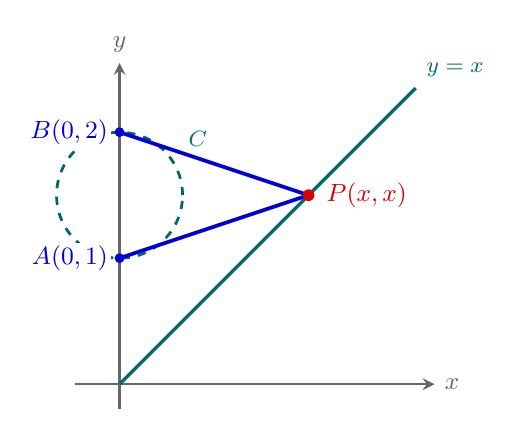
\begin{tikzpicture}[scale=1.6, >=stealth, every node/.style={font=\small}]
    \coordinate (O) at (0,0);
    \coordinate (A) at (0,1);
    \coordinate (B) at (0,2);
    \coordinate (P) at (1.5,1.5);
    \draw[->, gray!80!black, line width=0.9pt] (-0.35,0)--(2.5,0) node[right] {$x$};
    \draw[->, gray!80!black, line width=0.9pt] (0,-0.2)--(0,2.55) node[above] {$y$};
    \draw[dashed, teal!80!black, line width=1pt] (0,1.5) circle (0.5);
    \draw[teal!85!black, line width=1.25pt] (0,0)--(2.35,2.35)
    node[above right, font=\footnotesize] {$y=x$};
    \draw[blue!85!black, line width=1.35pt] (A)--(P)--(B);
    \node[circle, fill=blue!85!black, inner sep=1.25pt] at (A) {}; \node[blue!85!black, left=3pt, fill=white, inner sep=1pt] at (A) {$A(0,1)$};
    \node[circle, fill=blue!85!black, inner sep=1.25pt] at (B) {}; \node[blue!85!black, left=3pt, fill=white, inner sep=1pt] at (B) {$B(0,2)$};
    \node[circle, fill=red!85!black, inner sep=1.5pt] at (P) {}; \node[red!85!black, right=3pt] at (P) {$P(x,x)$};
    \node[teal!85!black, font=\footnotesize] at (0.62,1.95) {$C$};
  \end{tikzpicture}
  \caption{直線$y=x$上の点$P$と直径$AB$の円$C$}
\end{figure}

\end{document}
